 \subsection{Electronic chain linearity}

In order to prepare the data acquistion system, the entire electronical chain
was tested beforehand. In fact it is crucial that the response of each
electronic device used behaves linearly, as the information about the energy
of the incident particle must be univocally extracted at the end of the chain.

\bigbreak

\begin{figure}[h]
  \centering
  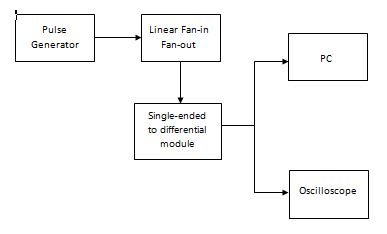
\includegraphics[scale=.5]{img/electronic_chain_diagram.JPG}
  \caption{The electronic chain}
  \label{chain}
\end{figure}

\bigbreak

The setup used is shown in Fig.~\ref{chain}. The output of a pulse generator (\num{100} ns square pulse of variable amplitude) is fed into a Fan-In Fan-Out module which reproduces the same signal for 12 channels. The signals are given in input to a ASIC charge-sensitive preamplifiers, designed by the INFN of Milan electonics group \cite{charge:amp}. These CSPs are realized in MAS 350 nm BiCMOS technology \cite{bicmos}. The chip is constituted by eight channels for anodic signals and one channel for cathodic ones, separately powered. The low-power design ensured a static power consuption under 12 mW per channel and the low-noise design allows for an equivalent input noise charge in the order of 125 electrons rms with 4 pF of detector capacitance. 

\bigbreak

The MDR/MDR cables had to be made in the laboratory as there was not enough AGATA cables for all the channels. Cables had been soldered manually and their ground had to be checked.
The output of the board as seen from the oscilloscope is shown in Fig.~\ref{osc}. The shape of the rising edge of the signal will be sampled during the acquisition from the detector in order to perform PSA on each event.

\bigbreak

\begin{figure}[h]
  \centering
  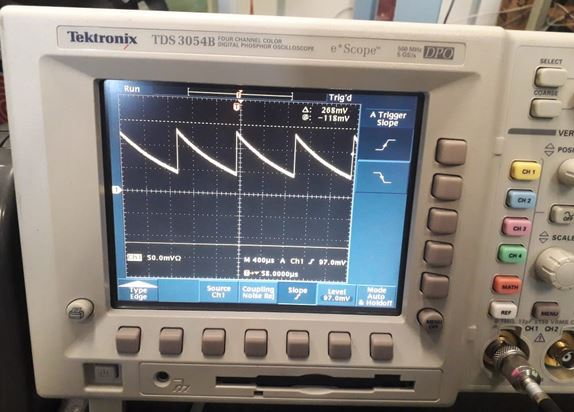
\includegraphics[scale=.35]{img/test_signal_oscilloscope.JPG}
  \caption{The output signal from the differential amplifier board, as seen on the oscilloscope.}
  \label{osc}
\end{figure}

\bigbreak

The signal from the preamiplifier is given to a 100 MHz 14-bit resolution digitizer throught a MDR-26 connector
The trapezoidal filter was applied to the signal through an FPGA with its charateristics \emph{risetime} and \emph{flat top} width parameters (Moving Windows Analysis)~\cite{salathe}. This step is crucial because the height of the peak from the differential amplifier board will be directly proportional to the energy of the incident particle in the detector. In the exponential curve of the signal, the amount of the time peak is present is very small and the peak detection is made difficult. By the differentiation of the signal, it is possibile to obtain the peak precisely and thus a trapezoidal signal is obtained. 
Hence, the height of the trapezoidal filter with the right parameters gives the information on the intensity of the peak available for longer time.

\bigbreak

The output of the trapezoidal filter is then sampled throught the acquisition software that also control the MWA variables. The software records the amplitude of the output and saves it into different channels during the time of the acquisition. A simple software, called TKT, is used to perform the fit on the peak obtained for the different pulse amplitude. 

\bigbreak

The linearity of the response of the boards is evalueted fitting the data obtained versus the voltage given as input to the preamplifier and checking the residuals plot as in Fig.~\ref{calib:plot:1} for all the 24 channels on the board.

\bigbreak

\begin{figure}[th]
  \centering
  \begin{minipage}[b]{0.45\textwidth}
    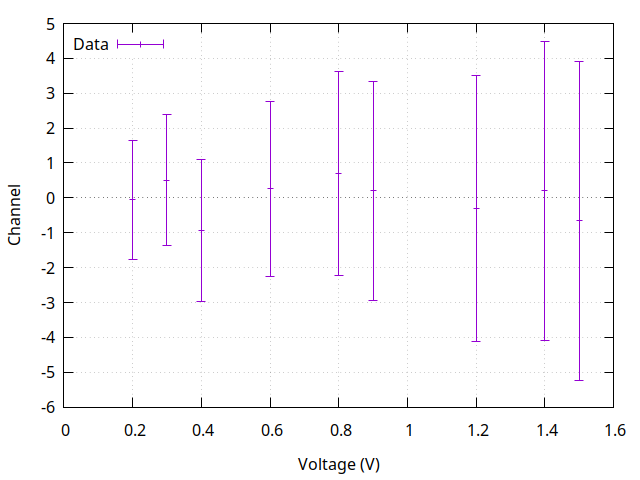
\includegraphics[width=\textwidth]{img/first_board_line/data_2/calib_1.png}
    \caption{Residual Plot for the the fit on the first channel on the tested board}
    \label{calib:plot:1}
  \end{minipage}
  \hfill
  \begin{minipage}[b]{0.45\textwidth}
  \begin{tabular}{lll}
    Voltage (V) & Channel & $\sigma$ \\
    \midrule
    0.2 & \num{393570.1} & 1.7 \\
    0.3 & \num{393753.2} & 1.8 \\
    0.4 & \num{393934.3} & 2.0 \\
    0.6 & \num{394300.5} & 2.5 \\
    0.8 & \num{394666.1} & 2.9 \\
    0.9 & \num{394848.1} & 3.1 \\
    1.2 & \num{395395.2} & 3.8 \\
    1.4 & \num{395760.8} & 4.3 \\
    1.5 & \num{395942.4} & 4.6 \\
    \bottomrule
  \end{tabular}
  \caption{Data for the fit}
  \label{calib:1}
  \end{minipage}
\end{figure}

\bigbreak

All the channels gave fairly similar results, therefore confirming the linearity of the response of the electronic chain and an overral well behavior of the differential board tested.

\subsection{Testing the TRACE detector}

In order to test the TRACE detector along with its preamplifier, it was put in a vacuum chamber, with a $\alpha$-ray source (Fig.~\ref{trace_chamber}).

\begin{figure}[h]
  \centering
  \includegraphics[scale=.05]{img/trace_chamber.jpg}
  \caption{The TRACE detector inside the chamber along with its preamplifier boards and the alpha source.}
  \label{trace_chamber}
\end{figure}

\bigbreak

To connect the integrated charge-sensitive pre-amplifiers to the TRACE silicon detector prototypes a custom board was designed and realized. Each board can host 2 ASIC pre-amplificators with 8 channels each. The ASICS can be reconfigured using different soldering in order to accept the back channel. As each detectors is segmented in 60 pads of 4 mm$^2$, a total of 4 pre-amplification boards are required by one telescope.
The amplified signals is going out of the chamber via a flat cable connected to a FISCHER 27-pins connectors feedthrough making the bridge between the reaction chamber under vacuum ($10^{-3}$ mbar) and the laboratory. Outside of the chamber, from each FISCHER connector, the cables are divided in two 12-pins MOLEX connectors mounted on the Single-ended-to-differential modules. From here the signal goes directly to the 14-bits 100 MHz digitizer for the GALILEO array using MDR-26 connectors and 10 m cables.

\bigbreak

The acquisition is triggered by the back portion of the detector, which is connected as Channel 0 of the digitizer, and it is performed as described in the former section. The resolution is tested using the three peaks of different sources (Tab.~\ref{peaks}). In Tab.~\ref{res:peaks:cab1} and Tab.~\ref{res:peaks:cab2} it is possible to see fit results for the $\alpha$ peaks for 2 different cables.

\begin{figure}[th]
  \centering
 \begin{tabular}{lc}
    Source & $E_\alpha$ (MeV)  \\ 
    \midrule
    \ce{^239Pu} & 5.1566  \\
    \ce{^241Am} & 5.4856  \\
    \ce{^244Cm} & 5.8048 \\
    \bottomrule
  \end{tabular}
  \caption{The predominant peaks from the triple-alpha source.}
  \label{peaks}
\end{figure}

\begin{figure}[h]
  \centering
  \begin{minipage}[b]{0.45\textwidth}
    \centering
  \begin{tabular}{ll}
    Channel & FWHM \\
    \midrule
    5150 & \num{29} \\
    5485 & \num{27} \\
    5804 & \num{25} \\
    \bottomrule
  \end{tabular}
  \caption{3-$\alpha$ peaks (cable 1)}
  \label{res:peaks:cab1}
  \end{minipage}
  \hfill
  \begin{minipage}[b]{0.45\textwidth}
    \centering
  \begin{tabular}{ll}
    Channel & FWHM \\
    \midrule
    5153 & \num{32} \\
    5485 & \num{27} \\
    5805 & \num{22} \\
    \bottomrule
  \end{tabular}
  \caption{3-$\alpha$ peaks (cable 2)}
  \label{res:peaks:cab2}
  \end{minipage}
\end{figure}

In Fig.~\ref{res:am}, Fig.~\ref{res:pu} and Fig.~\ref{res:cm} results of the calibration for different channels of the detector are shown. They are overral good throughout all the tested channels.

\begin{figure}[h]
  \centering
  \begin{minipage}[b]{0.45\textwidth}
  \vspace{5mm}
    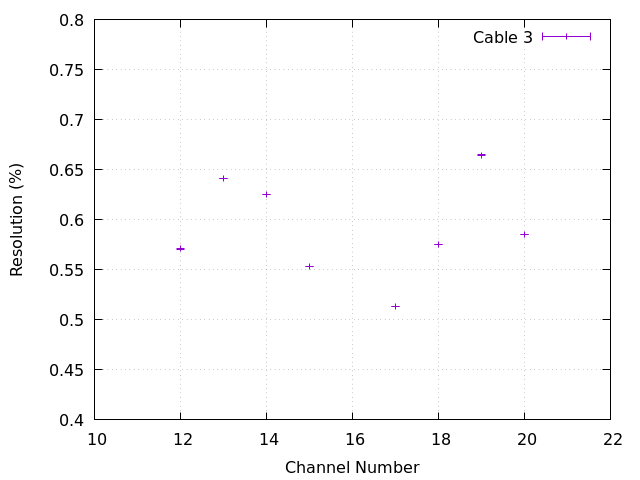
\includegraphics[width=\textwidth]{img/plot/am/3_res_am.png}
    %\caption{Resolution vs Channel}
    \label{res:am3}
  \end{minipage}
  \hfill
  \begin{minipage}[b]{0.45\textwidth}
    \begin{tabular}{lll}
      DAQ Channel & Resolution (\%) & $\sigma$ \\
      \midrule
      12 & \num{0.5708} & 0.0002 \\
      13 & \num{0.6413} & 0.0003 \\
      14 & \num{0.6253} & 0.0003 \\
      15 & \num{0.5535} & 0.0002 \\
      17 & \num{0.5131} & 0.0002 \\
      18 & \num{0.5752} & 0.0002 \\
      19 & \num{0.6646} & 0.0003 \\
      20 & \num{0.5854} & 0.0002 \\
      \bottomrule
    \end{tabular}
    \label{res:plot:am3}
  \end{minipage}
  \caption{Energy resolution (\%) of the TRACE detector for \ce{^241Am} peak.}
  \label{res:am}
\end{figure}

\begin{figure}[h]
  \centering
  \begin{minipage}[b]{0.45\textwidth}
  \vspace{5mm}
    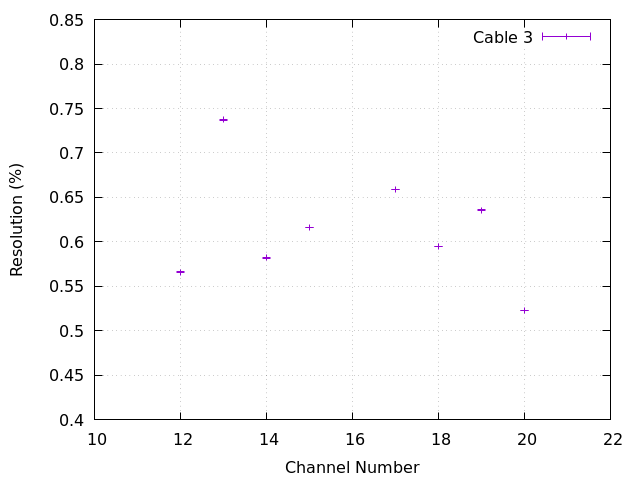
\includegraphics[width=\textwidth]{img/plot/pu/3_res_pu.png}
    %\caption{Resolution vs Channel}
    \label{res:pu3}
  \end{minipage}
  \hfill
  \begin{minipage}[b]{0.45\textwidth}
  \begin{tabular}{lll}
    DAQ Channel & Resolution (\%) & $\sigma$ \\
    \midrule
    12 & \num{0.5661} & 0.0003 \\
    13 & \num{0.7371} & 0.0003 \\
    14 & \num{0.5821} & 0.0003 \\
    15 & \num{0.6160} & 0.0003 \\
    17 & \num{0.6587} & 0.0003 \\
    18 & \num{0.5947} & 0.0003 \\
    19 & \num{0.6359} & 0.0003 \\
    20 & \num{0.5228} & 0.0002 \\
    \bottomrule
  \end{tabular}
  \label{res:plot:pu3}
  \end{minipage}
  \caption{Energy resolution (\%) of the TRACE detector for \ce{^239Pu} peak.}
  \label{res:pu}
\end{figure}

\begin{figure}[h]
  \centering
  \begin{minipage}[b]{0.45\textwidth}
  \vspace{5mm}
    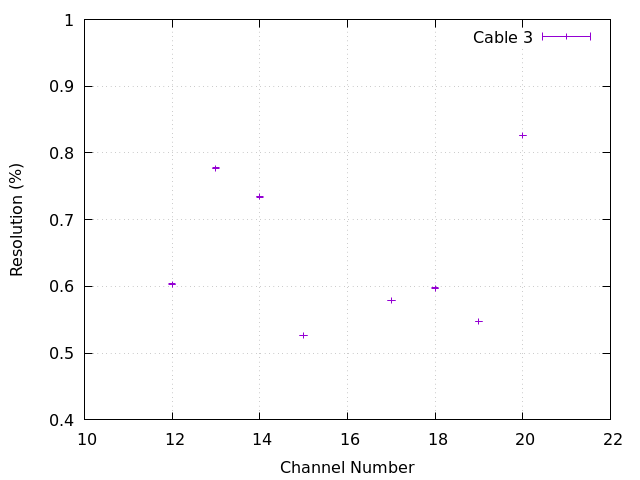
\includegraphics[width=\textwidth]{img/plot/cm/3_res_cm.png}
    %\caption{Resolution vs Channel}
    \label{res:cm3}
  \end{minipage}
  \hfill
  \begin{minipage}[b]{0.45\textwidth}
  \begin{tabular}{lll}
    DAQ Channel & Resolution (\%) & $\sigma$ \\
    \midrule
    12 & \num{0.6036} & 0.0003 \\
    13 & \num{0.7772} & 0.0004 \\
    14 & \num{0.7342} & 0.0004 \\
    15 & \num{0.5262} & 0.0002 \\
    17 & \num{0.5789} & 0.0003 \\
    18 & \num{0.5976} & 0.0002 \\
    19 & \num{0.5472} & 0.0002 \\
    20 & \num{0.8266} & 0.0002 \\
    \bottomrule
  \end{tabular}
  \label{res:plot:cm3}
  \end{minipage}
  \caption{Energy resolution (\%) of the TRACE detector for \ce{^244Cm} peak.}
  \label{res:cm}
\end{figure}

\clearpage

\subsection{GALTRACE experiment}

The experiment was performed in July 2019 at the Legnaro National Laboratory
(Italy). A \ce{^13C} beam, with energy of $23$ MeV and intensity around $1$ pnA
was focused on a $0.1$ mg/cm thick \ce{^19 F} -\ce{^7 Li} target, put on a base
made of \ce{^12 C}.
Two TRACE silicon detectors were placed inside the GALILEO HPGe array
scattering chamber. A common electrode covered the entire ohmic side of the
detector.

\bigbreak

Inside the chamber, the detectors were connected with a short cable to a
16-channel charge-sensitive preamplifier, designed at INFN Milano~\cite{strano}.
The preamplifier gain was $45$ mV/MeV yeilding a dynamic range of
approximately 100 MeV. The trigger of the acquisition was the signal from the
common electrode. The signals from one detector were sent to the digital
acquisition, while the second detector was connected to the analog read-out
line.

\bigbreak

The chain of the digital acquisition allowed to collect the signals (“traces”)
digitized by the 100 MHz sampling module. The length of the recorded trace was
1 $\mu$s, giving 100 points, at every 10 ns each. This length of the traces
was chosen to assure recording the full rise time on the one hand and at the
same time minimize the amount of written data. The signals were recorded,
digitized and afterwards processed to extract the relevant observables. The
placement of the TRACE module in the chamber with the ohmic side facing the
reaction products was important to enhance the PSA capability. The signals
were collected both from the ohmic side of the detector as well as from a few
groups of pads (or single pads).

\bigbreak

The trigger of the TRACE acquisition, obtained in this case from a digital
leading edge discriminator embedded in the module, was the signal from the
common electrode (“BACK”). The signals from the pads were collected only if
the BACK signal was present.

\subsection{Cabling Problem}

After the data acquisition period, a problem with digitizer cabling was
discovered. In fact the two digitizer used for the TRACE detector
(\textit{gal09} and \textit{gal10}) did not use the same MDR cables. All the
channels, apart from 17 to 24 ones of the \textit{gal10}, were connected through
high-end AGATA 10m MDR/MDR cables used by previous experiment. As there were
not enough cables, all the others channels were connected through home made
MDR cables constructed in the LNL laboratory specifically for this experiment.

\bigbreak

In the Fig.~\ref{cable} it is possible to see the differences in the Pulse
Shape of the signals from different types of cables, which are enumerated in
the Tab.~\ref{cables}. As the analysis is made using the Pulse Shape Analysis
(PSA), small differences in the signal propagation has to be taken into
account when calculating the discriminating variables. In fact, as it is clear
from the plot, the rise time and the maximum derivative of the signal will be
different for different types of cable, thus preventing the use of the same
cuts and the same Neural Network model for the PSA.

\bigbreak

\begin{figure}[h]
  \centering
  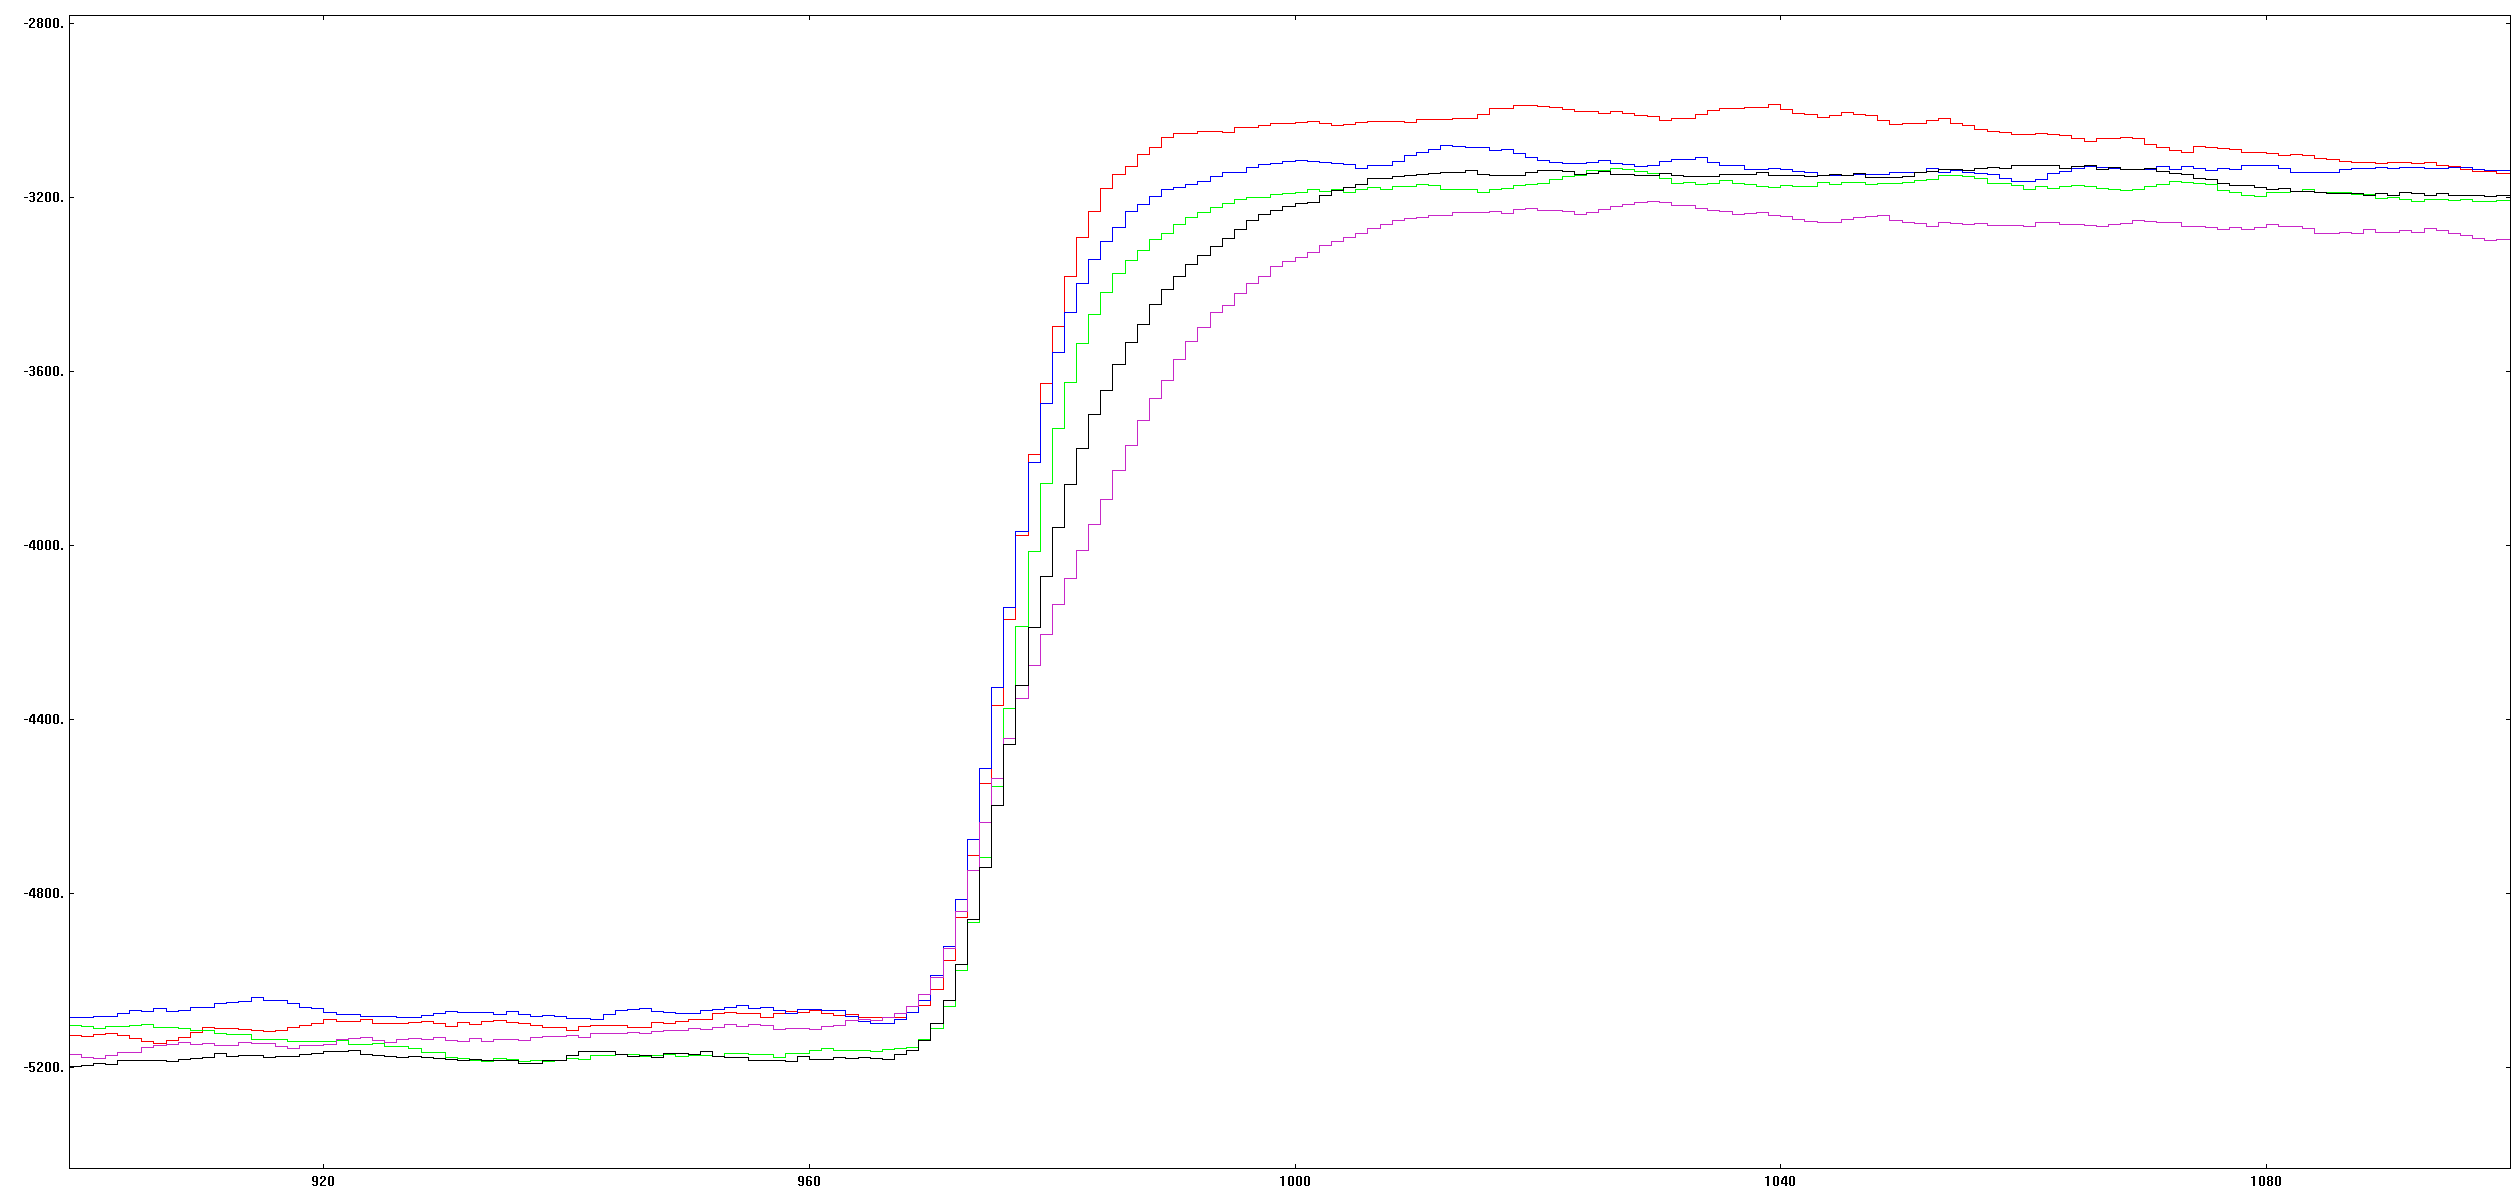
\includegraphics[scale=.16]{img/cabling.png}
  \caption{TRACE signals from different cable type.}
  \label{cable}
\end{figure}

\begin{figure}
  \begin{tabular}{ll}
    Signal Color & Cable \\
    \midrule
    Red & GALILEO 0.8m MDR/MDR \\
    Blue & AGATA 10m MDR/MDR \\
    Green & AGATA 10m MDR/MDR (previous generation 3M cable) \\
    Magenta & Home made MDR flat cables \\
    Black & New cable for TRACE \\
    \bottomrule
  \end{tabular}
  \label{cables}
\end{figure}

\bigbreak

In order to make up for this, the \textit{gal10} 17-24 channels were analyzed
separately, making different cuts and creating a specific Neural Network model
for those. In this way it is possible to discriminate successfully the
protons and $\alpha$ signals also for channels connected through different MDR
cables.